\documentclass{article}
\usepackage[utf8]{inputenc}
\usepackage[american, siunitx]{circuitikz}
\usepackage{ulem}
\usepackage{float}
% \usepackage{url}
\usepackage{hyperref}

\title{555 Timer as Astable Multivibrator}
\author{Scott Morgan}
\date{Rev. December 9, 2022}

\begin{document}

\begin{figure}[H]
    \centering

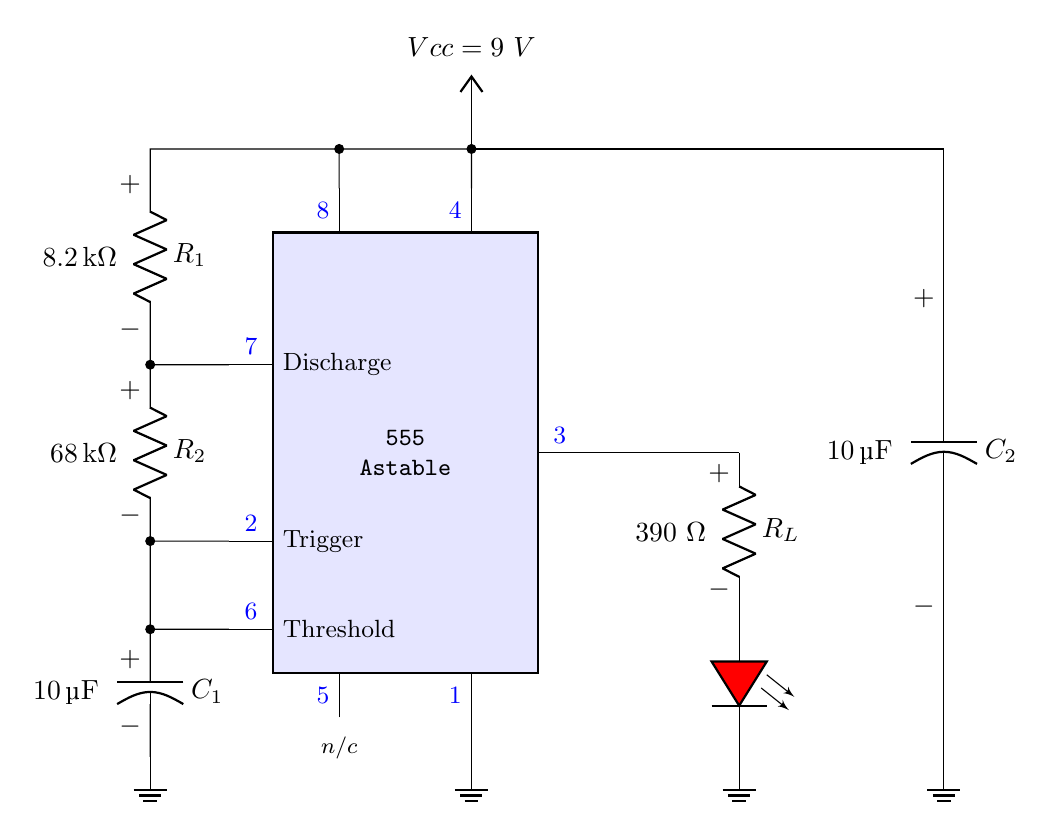
\begin{tikzpicture}[]
%------------------------------------------------------------------------------------------------
% 555 Symbol Definition

    \tikzset{ic555/.style={muxdemux,
            muxdemux def={Lh=10, NL=5, Rh=10, NR=5,
            NB=2, w=6, NT=2, square pins=1},
        no input leads, external pins width=0.4,
        circuitikz/muxdemuxes/fill=blue!10}
    }
    \node [ic555, font=\small\ttfamily,align=center](A) at (0,0) {555\\Astable};
    % left pins
    \foreach \rawpin/\npin/\label in {2/7/Discharge, 4/2/Trigger, 5/6/Threshold} {
        \draw (A.lpin \rawpin) coordinate(\label) -- (A.blpin \rawpin)
            node[midway, blue, font=\small, above]{\npin}
            node[right, font=\small]{\label};
    }
    % top pins
    \foreach \rawpin/\npin/\label in {1/8/vcc, 2/4/reset} {
        \draw (A.tpin \rawpin) coordinate(\label) -- (A.btpin \rawpin)
            node[midway, blue, font=\small, left]{\npin};
    }
    % bottom pins
    \foreach \rawpin/\npin/\label in {1/5/control, 2/1/ground} {
        \draw (A.bpin \rawpin) coordinate(\label) -- (A.bbpin \rawpin)
            node[midway, blue, font=\small, left]{\npin};
    }
    % finally, left
    \draw (A.rpin 3) coordinate(output) -- (A.brpin 3) node[midway, blue, font=\small, above]{3};   
%------------------------------------------------------------------------------------------------
\draw (ground) -- ++(0, -0.5) coordinate(commongnd) node[ground]{} ;

\draw (reset) to[short, -*] ++(0, 0.5) coordinate(top) to[short, -*] (top -| vcc) ; 
\draw (vcc) -- (top -| vcc) -- (top -| Discharge) -- ++(-1, 0) coordinate(left) to[R, v=8.2<\kilo\ohm>, 
l=$R_1$,-*] (Discharge -| left) -- (Discharge);
\draw (left |- Discharge) to[R, v=68<\kilo\ohm>, l=$R_2$, -*] (left |- Trigger) -- (Trigger);
\draw (left |- Trigger) to[short,-*] (left |- Threshold) -- (Threshold); 
\draw (left |- Threshold) to[curved capacitor, v=10<\micro\farad>, l=$C_1$] (left |- commongnd) node[ground]{};
\draw (control)  node[label={[font=\footnotesize]below:$n/c$}] {};
\draw (top) to[short] ++(0, 0.5) node[vcc] {$Vcc=9\ V$};
\draw (output) -- ++(2,0) coordinate(output2);
\draw (output2) to[R, v=$390\ \Omega$, l=$R_L$] ++(0, -2) to [led, fill=red] (output2 |- commongnd) node[ground] {};
\draw (top) -- ++(6,0) coordinate(topC2) to[curved capacitor, v=10<\micro\farad>, l=$C_2$] (topC2 |- commongnd) node[ground] {}; 
    
\end{tikzpicture}
    \caption{555 timer configured as an astable multivibrator.}
    \label{fig:astable}
\end{figure}

\end{document}
